\documentclass[xcolor={dvipsnames}]{beamer}
\usepackage{color, colortbl}
\usepackage{transparent}
\usepackage[ngerman,english]{babel}
\usepackage[T1]{fontenc}
\usepackage{lmodern}
%\usepackage{subfigure}
%\usepackage[compatibility=false]{caption}
%\usepackage{subcaption}
\usepackage{tikz}
\usepackage{textgreek}
\usepackage{tabularx}
\usepackage{booktabs}
\usepackage{siunitx}
\usepackage{units}
\usepackage[absolute,overlay]{textpos} %for positioning the logos where I want

\mode<presentation>
{
  \usetheme{CambridgeUS}     
  \usecolortheme{lily} 
  \definecolor{beamer@violet}{rgb}{0.5,0.3,0.5} % changed this
  \setbeamercolor{structure}{fg=beamer@violet!70!cyan}
  \setbeamercolor{palette primary}{fg=black, bg=gray!30!white!50!cyan!20!}
  \setbeamercolor{palette secondary}{fg=black, bg=gray!30!white!30!cyan!40!}
  \setbeamercolor*{palette tertiary}{bg=gray!20!white!20!cyan!60!}
  
  \setbeamercolor{frametitle}{fg=cyan!60!white!40!,bg=cyan!80!black}
  \setbeamercolor{title}{fg=cyan!80!black}
  \setbeamercolor{normal text}{fg=black,bg=white}
  \setbeamercolor{alerted text}{fg=beamer@violet}
  \setbeamercolor{example text}{fg=beamer@violet!70!cyan}
  
  \usefonttheme{structureitalicserif} 
  \setbeamertemplate{navigation symbols}{}
  \setbeamertemplate{caption}[numbered]
} 

\newcommand{\sidlogo}{
  \setlength{\TPHorizModule}{1pt}
  \setlength{\TPVertModule}{1pt}
   % textblock{}{x,y}: pos(x) = rightUpperCorner + (x * \TPHorizModule), pos(y) = leftUpperCorner - (y * \TPVertModule)
  \begin{textblock}{1}(323,12)
   
\includegraphics[width=40pt,height=26pt]{figures/SiD.jpeg}
  \end{textblock}
  } 
\newcommand{\ilclogo}{
  \setlength{\TPHorizModule}{1pt}
  \setlength{\TPVertModule}{1pt}
   % textblock{}{x,y}: pos(x) = rightUpperCorner + (x * \TPHorizModule), pos(y) = leftUpperCorner - (y * \TPVertModule)
  \begin{textblock}{1}(323,12)
   
\includegraphics[width=40pt,height=26pt]{figures/ILC.jpeg}
  \end{textblock}
} 

\title[ILC \& Pair Background Envelopes]{\textbf{\LARGE Pair Background Envelopes} \\ \vspace*{0.3cm} \small LCWS Morioka}
\author[Anne Sch\"utz]{\textbf{Anne Sch\"utz}}
\institute{\textbf{DESY}}
\date{\textbf{7th December 2016}}

\titlegraphic{
\includegraphics[height=1.0cm]{figures/SiD.jpeg}\hspace*{6cm}~%
   
\includegraphics[height=1.0cm]{figures/DESY_Logo.png}
}

\begin{document}
{
\usebackgroundtemplate{
 \tikz\node[opacity=0.1]{\hspace*{-.05in}\vspace*{-4in}{\transparent{0.1}\includegraphics[width=\paperwidth]{figures/Helix_tracks.pdf}}};
 % \tikz\node[opacity=0.2]{\centering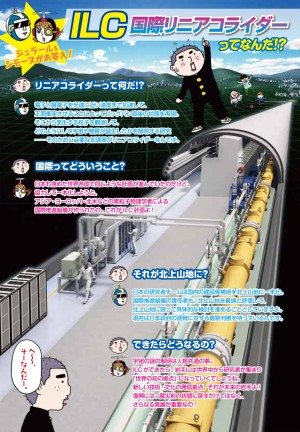
\includegraphics[height=\paperheight]{Iwatecomics.jpg}};
 }
\begin{frame}
  \titlepage
\end{frame}
}
\begin{frame}
  \tableofcontents
\end{frame}

\section{Pair background envelope by Takashi Maruyama}
\begin{frame}
\begin{center}
  \includegraphics[height=0.9\textheight]{slide_takashi.jpg}
\end{center}
 \begin{flushright} 
  (Takashi Maruyama, 2007)
 \end{flushright}
\end{frame}
\begin{frame}{Method}
 In an e-mail correspondence, Takashi said:
 \begin{itemize}
 \item Because of limited CPU power he only wanted to plot particles with tracks on the envelope.
 \item He used the fit function $P_T = a*p_z^b$, with a and b being dependent on the beam parameters.
\end{itemize}
\end{frame}

\section{Pair background envelopes with GuineaPig pairs}
\subsection{Method}
\begin{frame}{Helix Algorithm}
\ilclogo
I did not apply any cuts on the data set.\\
The algorithm takes as arguments:
\begin{itemize}
 \item Particle vertices
 \item Momenta
 \item Charge
\end{itemize}

Then it calculates:
\begin{itemize}
 \item Radius of the projected circle
 \item Center position of the circle
 \item Pitch of the helix
\end{itemize}

Assumptions:
\begin{itemize}
 \item In the region shown, the momenta of the particles do not changed.
 \item The radius of the helices is hence constant over this distance.
 \item Interactions with other particles/material is not taken into account.
\end{itemize}
\end{frame}

\subsection{Results}
\begin{frame}{The helix envelopes in the XZ plane}
\ilclogo
Pair helixes from 1 bunch crossing are drawn:\\
\vspace*{0.2cm}
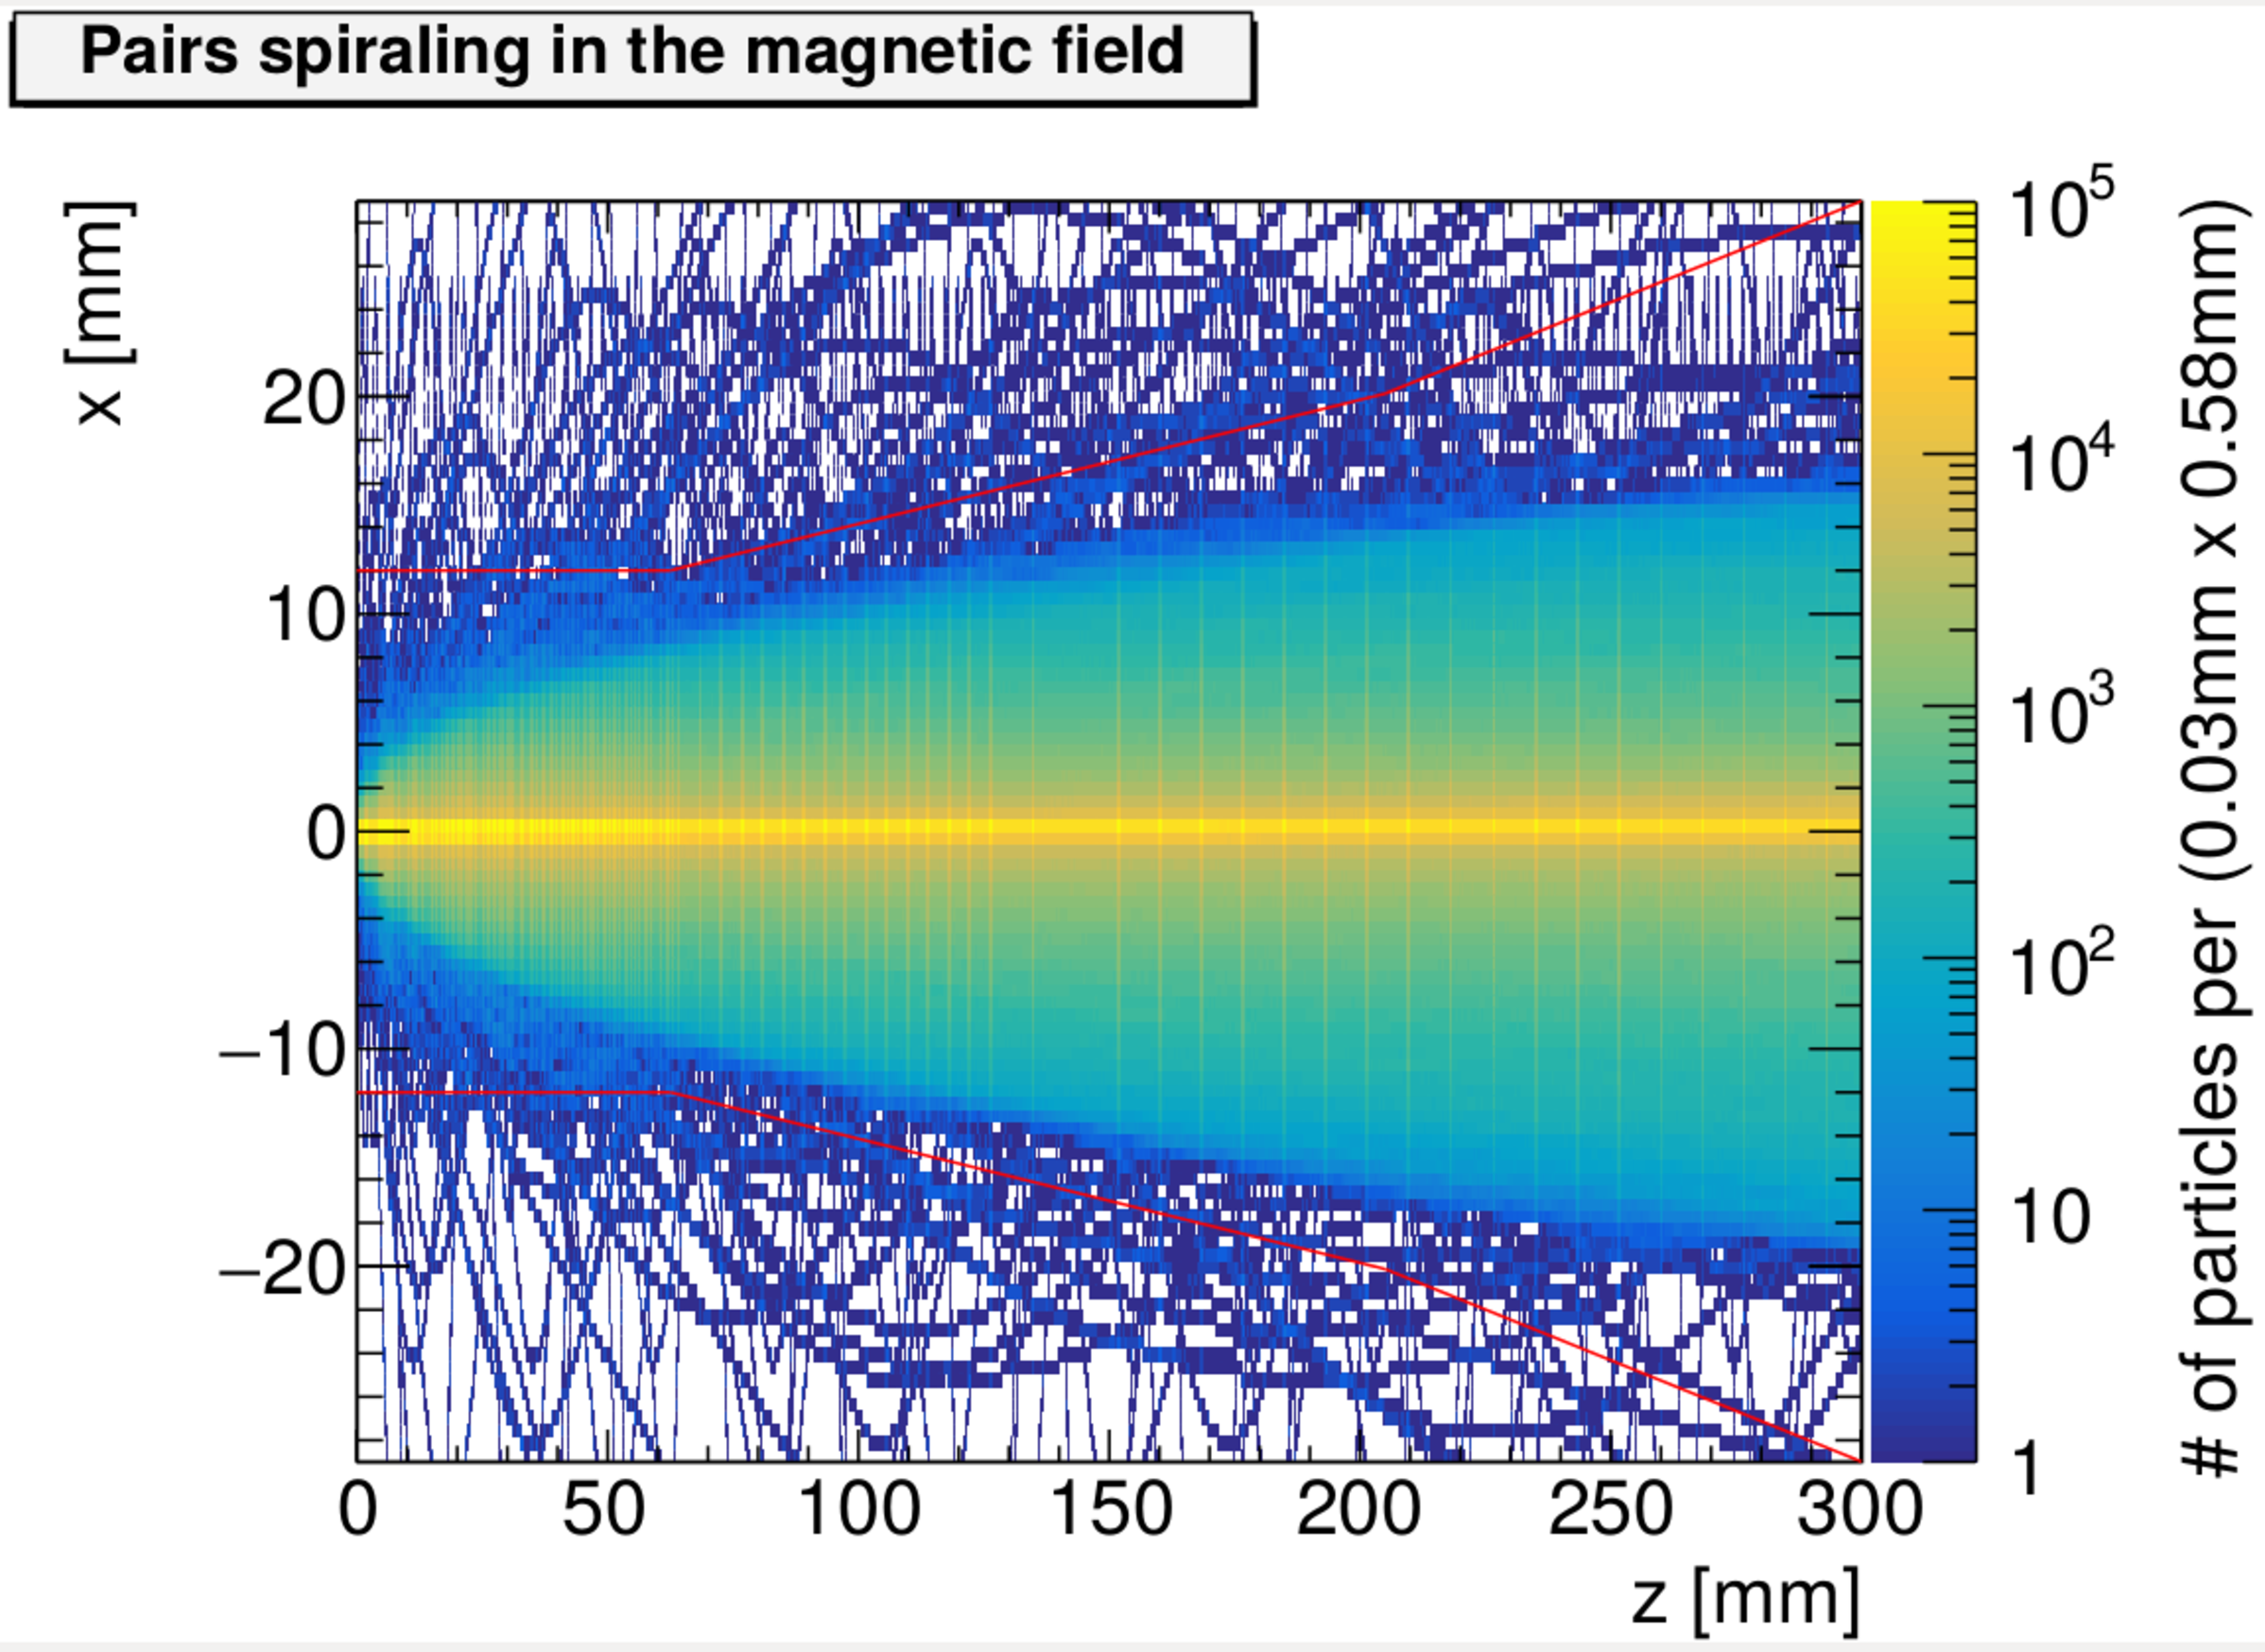
\includegraphics[width=0.52\textwidth]{figures/Helix_tracks_xz_1bunch_lowres.pdf}
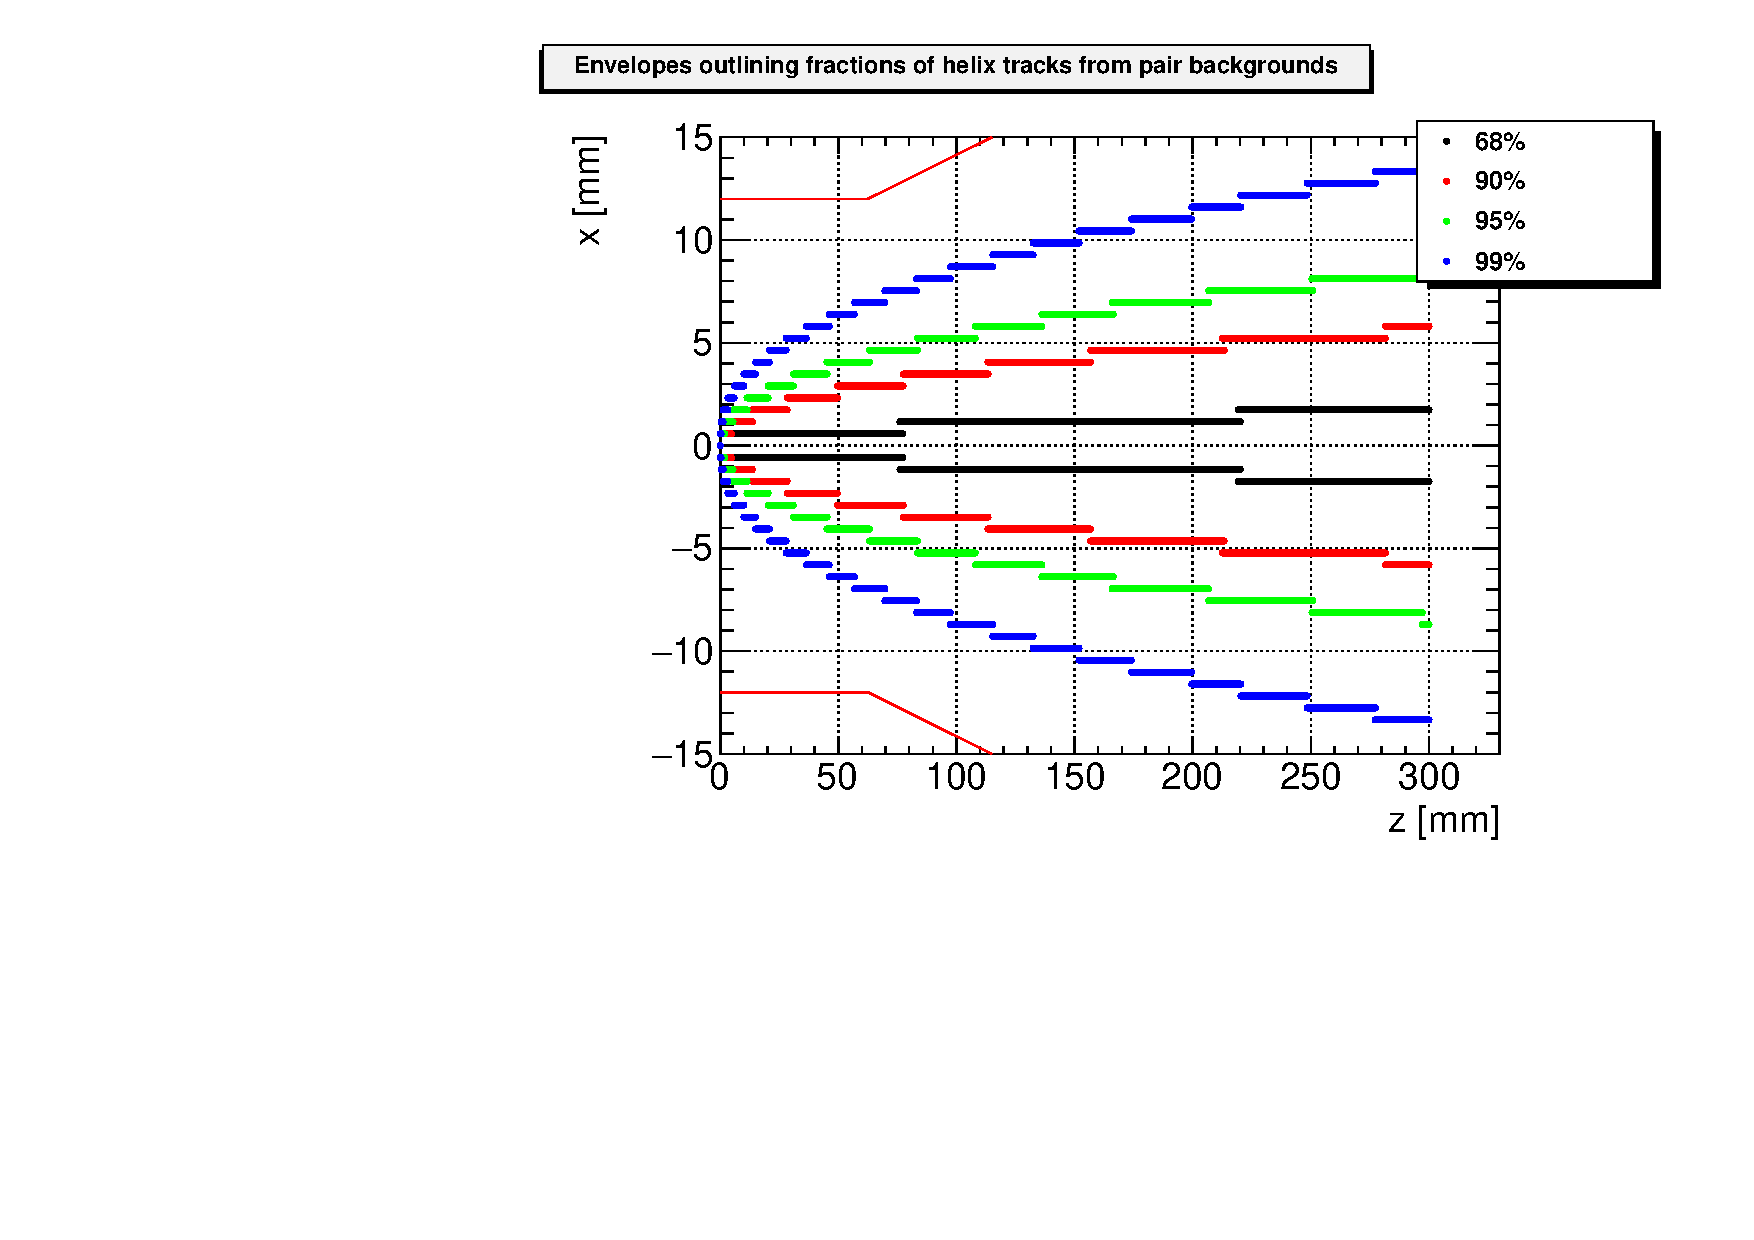
\includegraphics[width=0.52\textwidth]{figures/HelixEnvelopes_xz.pdf}
\end{frame}
\begin{frame}{The helix envelopes in the YZ plane}
\ilclogo
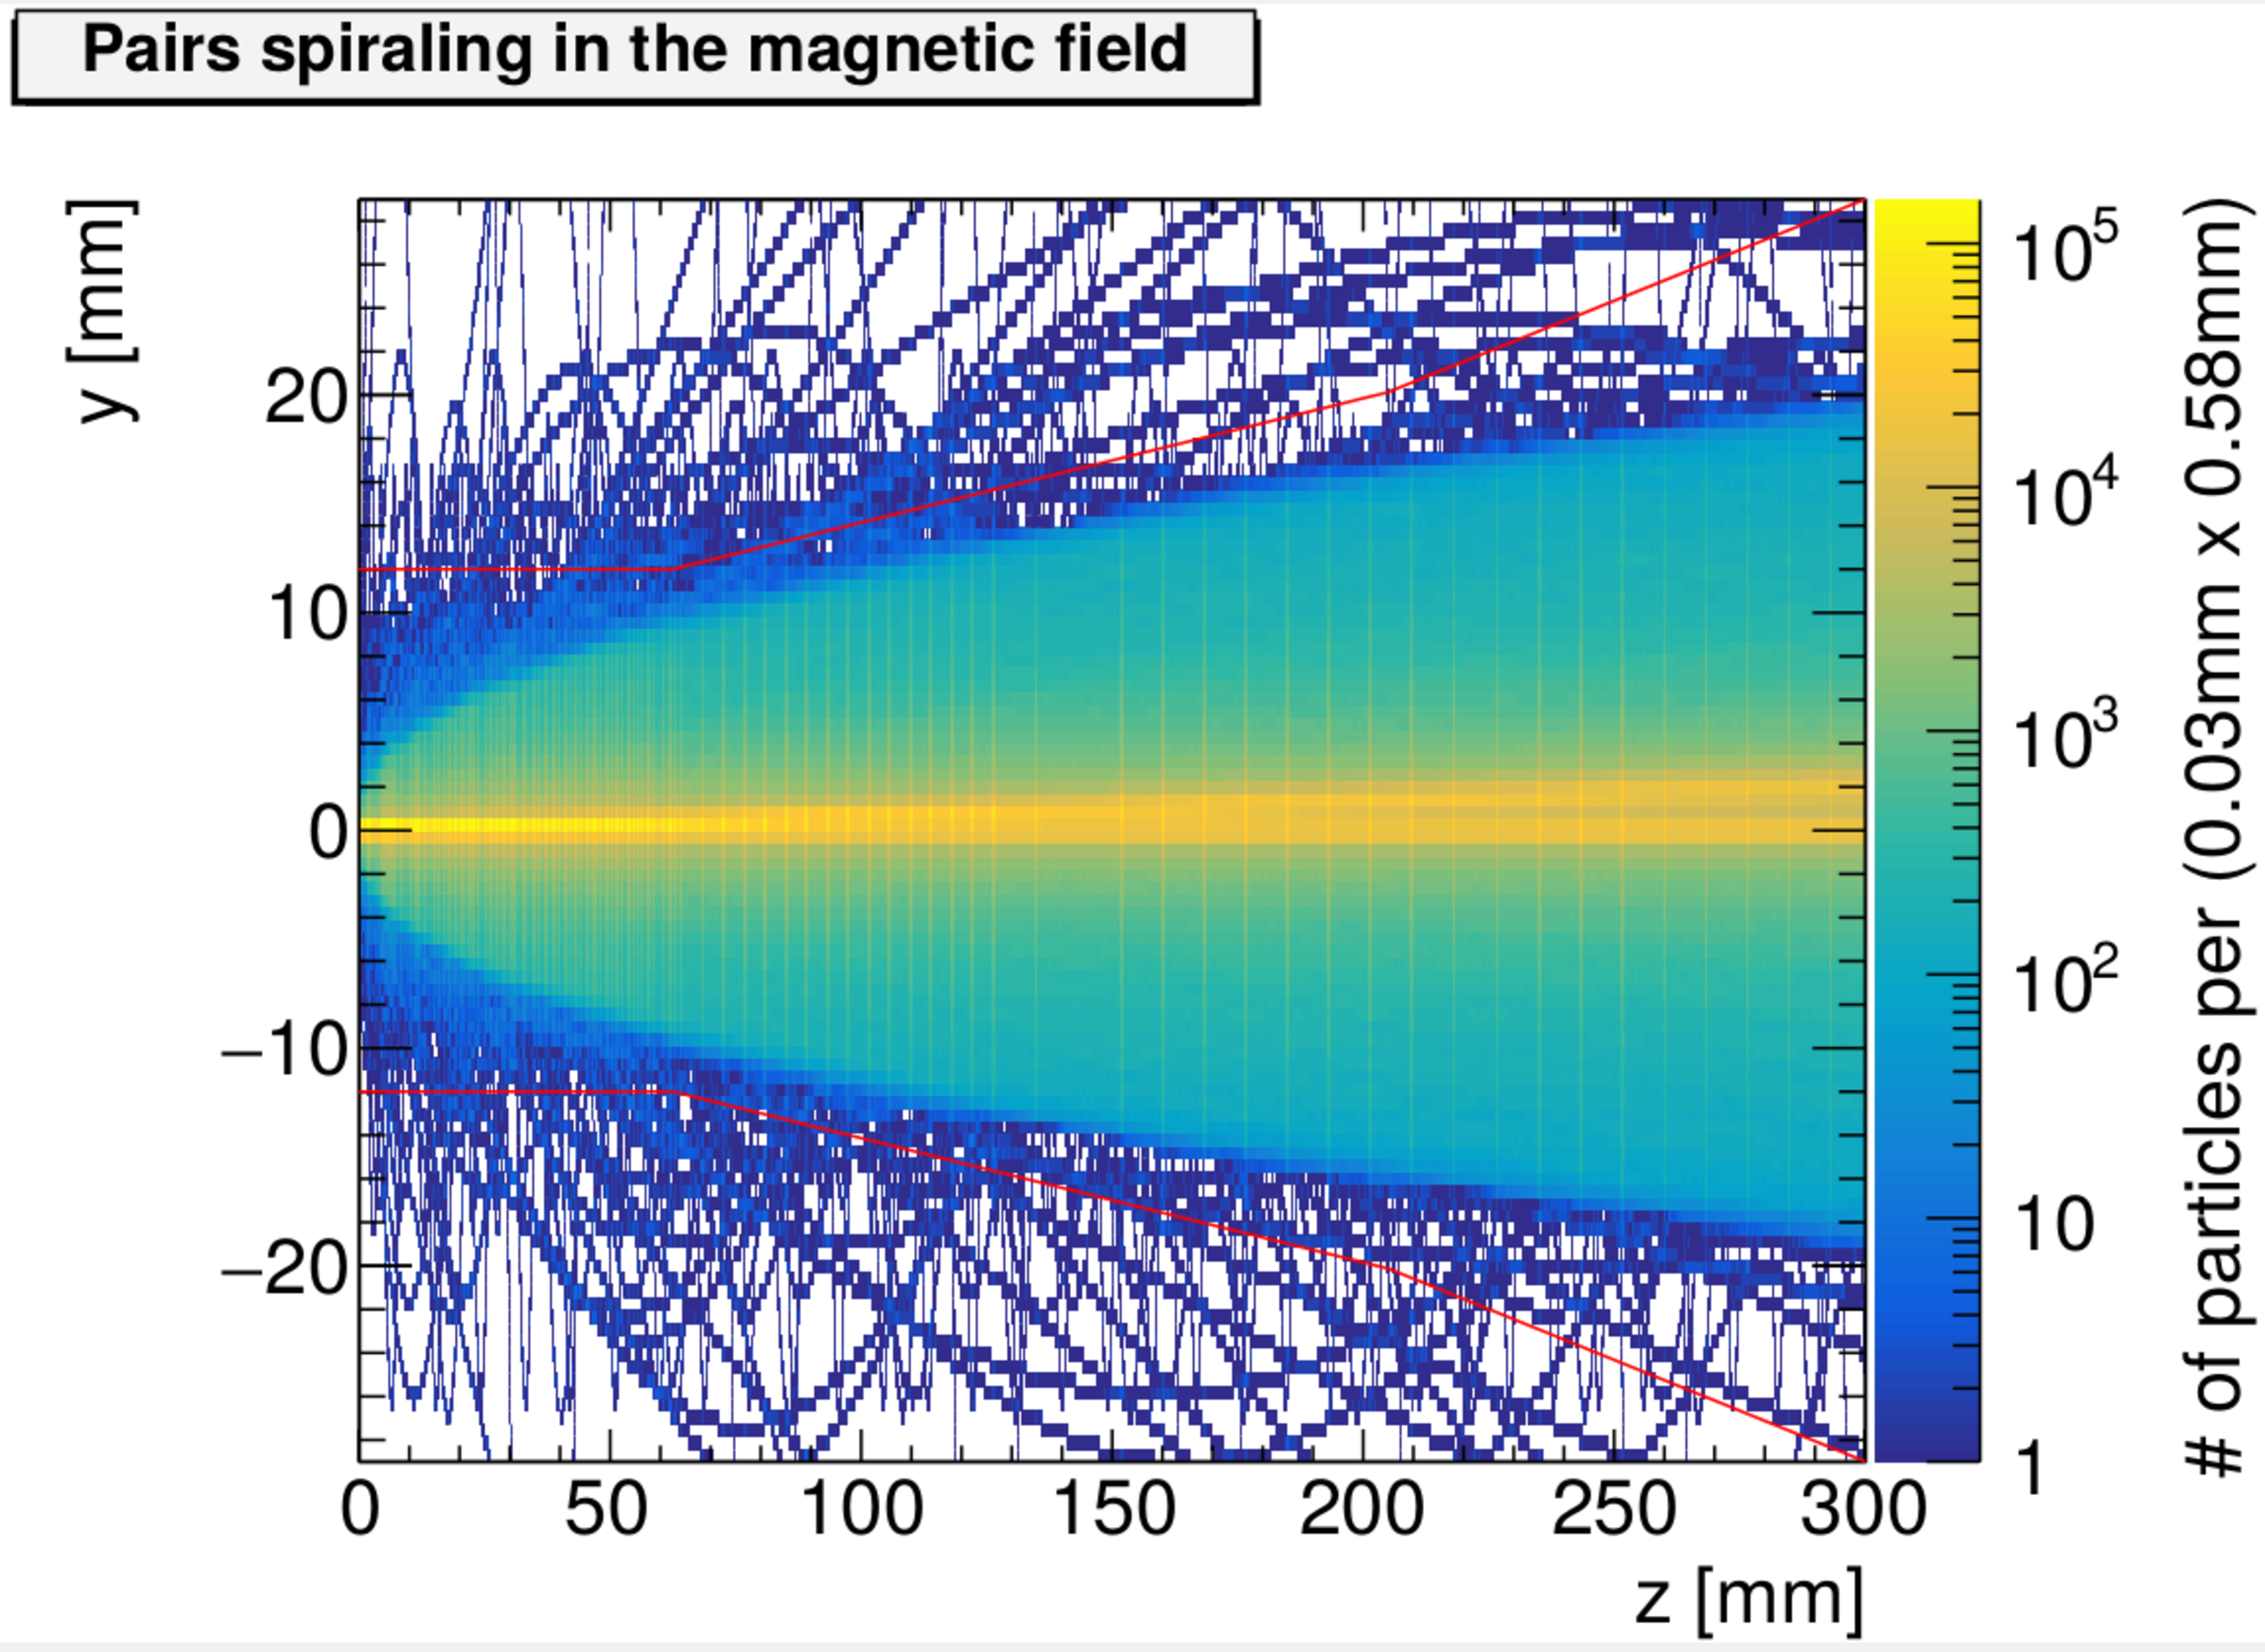
\includegraphics[width=0.52\textwidth]{figures/Helix_tracks_yz_1bunch_lowres.pdf}
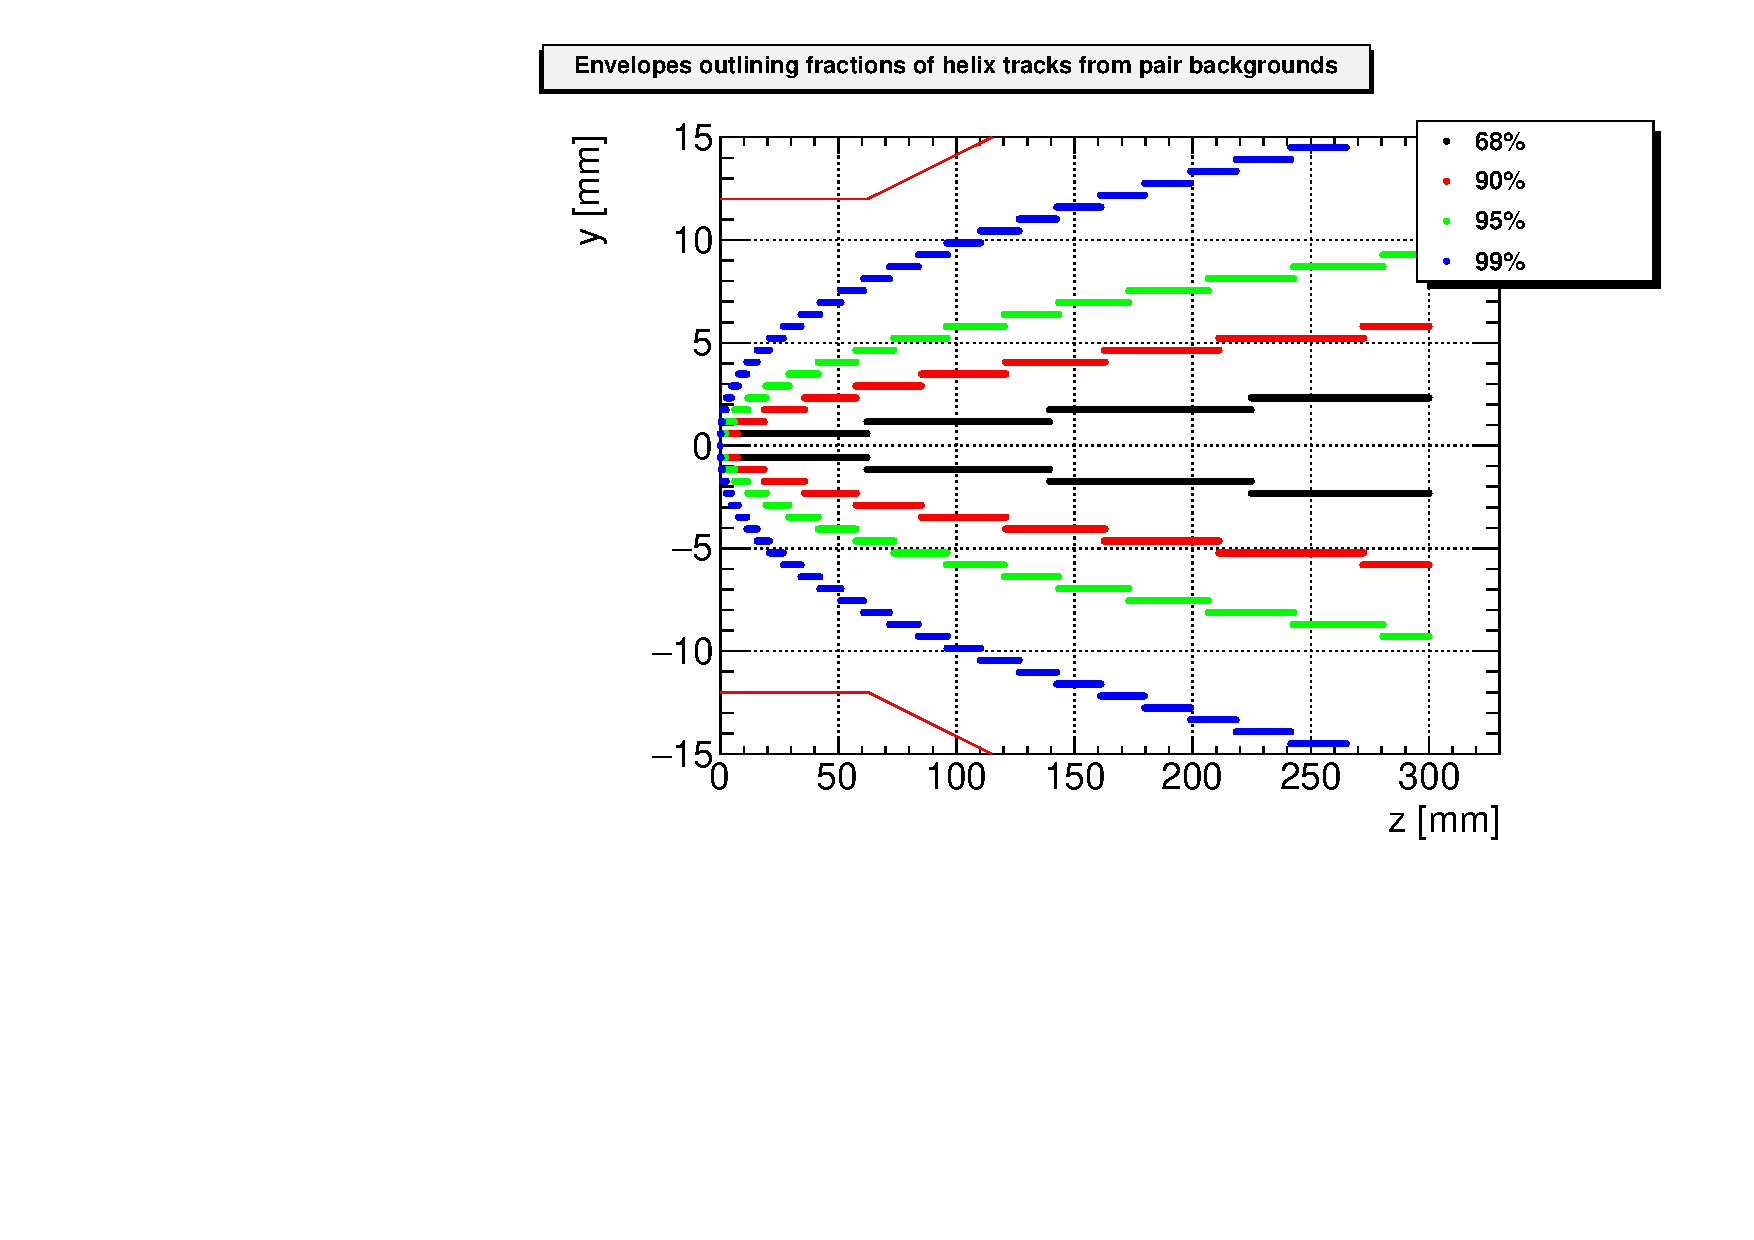
\includegraphics[width=0.52\textwidth]{figures/HelixEnvelopes_yz.pdf}\\
The distribution is broader in the YZ-plane because the x-momentum distributions are broader.
The asymmetry in y is due to the different momenta of positrons and electrons for positive z.
\end{frame}

\section{Conclusion}
\begin{frame}{Conclusion}
\begin{itemize}
 \item With the current beam pipe design, \textbf{only $\sim$ 0.45\%} of all pairs leave tracks \textbf{outside the beam pipe}.
 \item We could think about \textbf{reducing the beam pipe radius by 2\,mm}.
 \item We could think about \textbf{adding another vertex detector layer} with smaller radius.
\end{itemize}
BUT:
It needs to be studied how big the \textbf{advantage for e.g. c-tagging} is,
and what the \textbf{level of background/synchrotron radiation is at such radii}.
 
\end{frame}

%%--------------------------------------------------------------------------------
\section*{Appendix}
\begin{frame}
 \begin{center}
  Appendix
 \end{center}
\end{frame}

\subsection*{Pair particle momenta}
\begin{frame}{Plots of the pair momenta}
\sidlogo
 \begin{center}
 \hspace*{0.5cm} Electrons \hspace*{4.5cm} Positrons
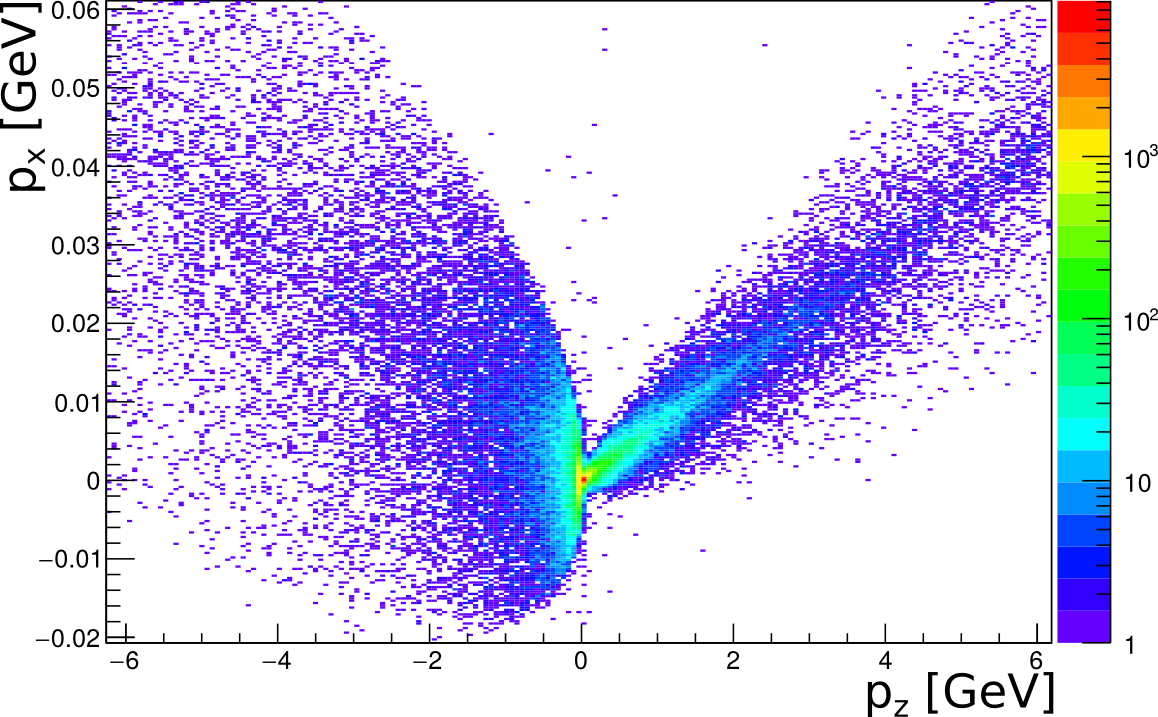
\includegraphics[width=0.52\textwidth]{figures/Momentumx_Momentumz.pdf}
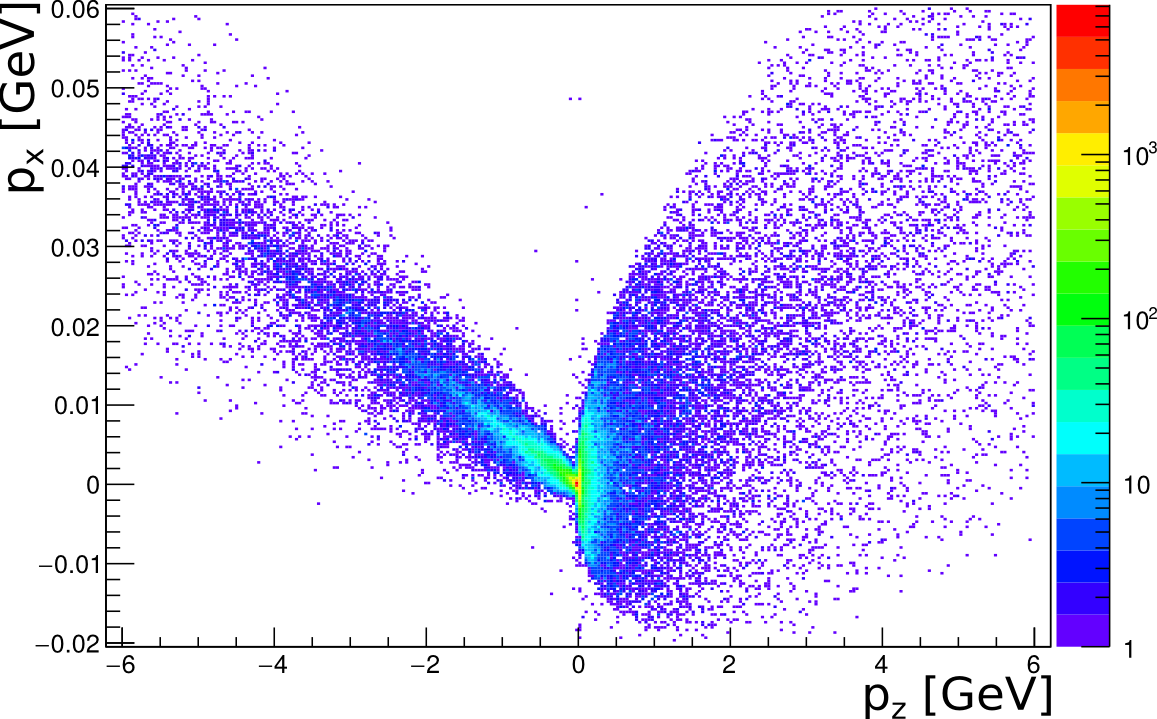
\includegraphics[width=0.52\textwidth]{figures/Momentumx_Momentumz_Positrons.pdf}
\end{center}
\end{frame}
\begin{frame}{Plots of the pair momenta}
\sidlogo
 \begin{center}
 \hspace*{0.5cm} Electrons \hspace*{4.5cm} Positrons
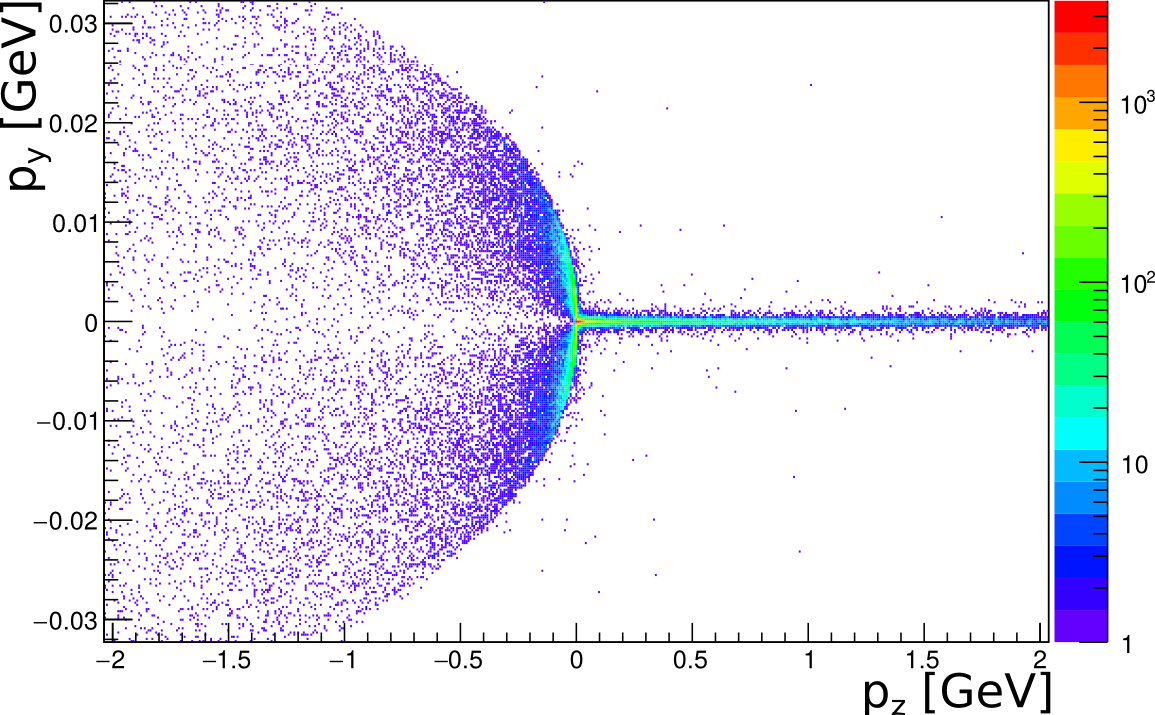
\includegraphics[width=0.52\textwidth]{figures/Momentumy_Momentumz.pdf}
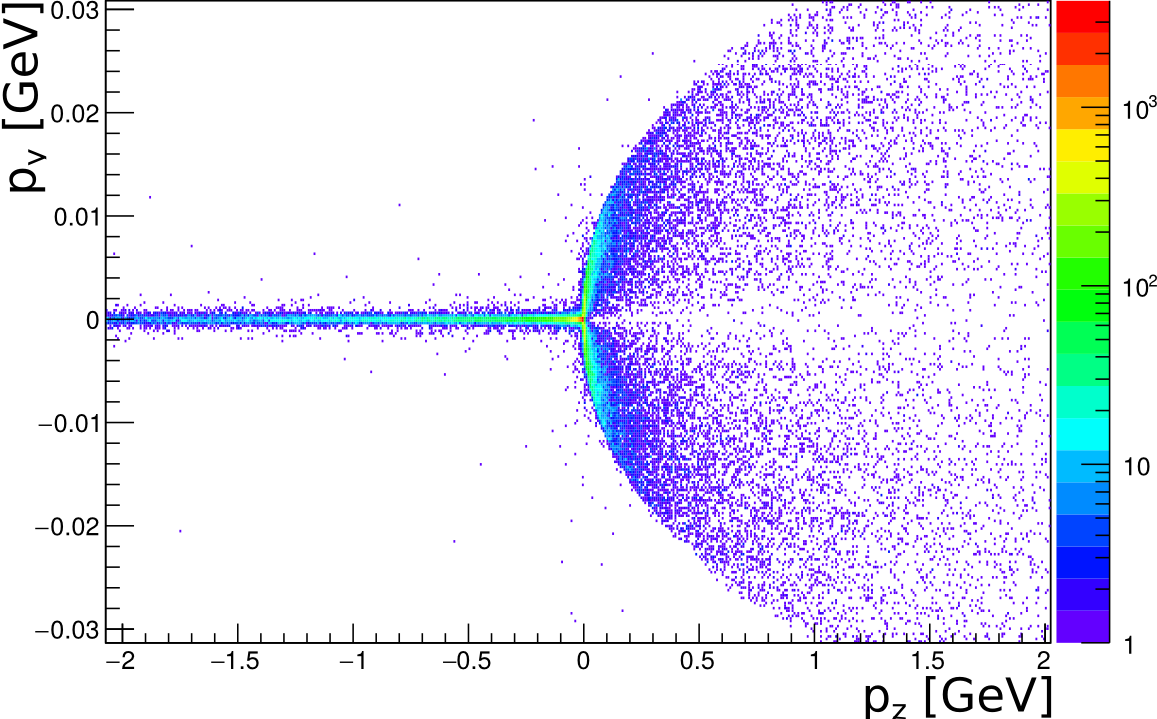
\includegraphics[width=0.52\textwidth]{figures/Momentumy_Momentumz_Positrons.pdf}
\end{center}
\end{frame}
\subsection*{Scheme of the helix projection on the XY-plane}
\begin{frame}
\sidlogo
 \begin{center}
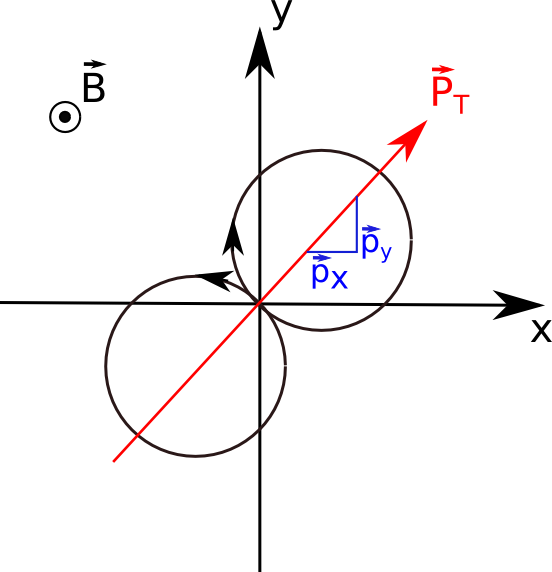
\includegraphics[width=0.65\textwidth]{figures/Helix_explanation.png}
\end{center}
\end{frame}

\end{document}
